\secnumberlesssection{ANEXOS}

En los Anexos se incluye todo aquel material complementario que no es parte del contenido de los capítulos de la memoria, pero que permiten a un lector contar con un contenido adjunto relacionado con el tema.

\subsection{ANEXO A: RESULTADOS DE VALIDACIÓN - BAJAS FRECUENCIAS (FRB 121102)}

\subsubsection{Bursts Confirmados por Literatura}

\begin{table}[H]
    \centering
    \caption{Bursts de FRB121102 confirmados por literatura (detectados por DRAFTS++ y reportados por Cruces et al. 2020). \textit{Fuente: Elaboración propia basada en Cruces et al. (2020) \cite{cruces2020frb121102}.}}
    \label{tab:anexo_confirmed_bursts}
    \begin{tabular}{|c|c|c|c|c|c|c|c|}
        \hline
        \multicolumn{4}{|c|}{\textbf{Columna 1}} & \multicolumn{4}{|c|}{\textbf{Columna 2}} \\
        \hline
        \textbf{File} & \textbf{DM} & \textbf{Time(s)} & \textbf{MJD} & \textbf{File} & \textbf{DM} & \textbf{Time(s)} & \textbf{MJD} \\
        \hline
        3096 & 564.15 & 114.059783 & 58440.83884126 & 3100 & 565.97 & 1253.032154 & 58441.01915005 \\
        3096 & 564.64 & 2172.299182 & 58440.86266456 & 3100 & 564.96 & 2090.123919 & 58441.02883908 \\
        3098 & 564.77 & 229.680524 & 58440.92373659 & 3100 & 557.7 & 2090.126104 & 58441.02883929 \\
        3098 & 565.35 & 1359.279991 & 58440.93681124 & 3100 & 563.53 & 2172.314365 & 58441.02979044 \\
        3098 & 563.5 & 3445.629 & 58440.96095990 & 3101 & 558.49 & 1160.627268 & 58441.05983026 \\
        3099 & 557.55 & 2331.324798 & 58440.98983520 & 3101 & 557.92 & 1174.354439 & 58441.05998916 \\
        3099 & 564.17 & 3111.182227 & 58440.99886157 & 3101 & 558.01 & 1297.028219 & 58441.06140906 \\
        3100 & 565.38 & 254.527406 & 58441.00759278 & 3101 & 566.12 & 1571.448422 & 58441.06458515 \\
        3100 & 557.11 & 310.032903 & 58441.00823545 & 3101 & 565.31 & 1814.433191 & 58441.06739762 \\
        3100 & 563.91 & 686.839999 & 58441.01259666 & 3102 & 563.14 & 1571.362789 & 58441.10636851 \\
        3100 & 564.75 & 942.375786 & 58441.01555436 & 3102 & 556.67 & 1823.937659 & 58441.10929213 \\
        3100 & 563.87 & 1148.701027 & 58441.01794252 & 3102 & 563.94 & 2099.014533 & 58441.11247584 \\
        \hline
    \end{tabular}
\end{table}

\subsubsection{Nuevos Candidatos Sin Confirmar}

\begin{table}[H]
    \centering
    \caption{Nuevos candidatos a bursts detectados únicamente por DRAFTS++ (pendientes de confirmación científica). \textit{Fuente: Elaboración propia}.}
    \label{tab:anexo_candidate_bursts}
    \begin{tabular}{|c|c|c|c|c|c|c|c|}
        \hline
        \multicolumn{4}{|c|}{\textbf{Columna 1}} & \multicolumn{4}{|c|}{\textbf{Columna 2}} \\
        \hline
        \textbf{File} & \textbf{DM} & \textbf{Time(s)} & \textbf{MJD} & \textbf{File} & \textbf{DM} & \textbf{Time(s)} & \textbf{MJD} \\
        \hline
        3096 & 579.6 & 1208.742 & 58440.851511757 & 3100 & 260.22 & 3037.433692 & 58441.03980380 \\
        3096 & 565.46 & 2789.205716 & 58440.86980499 & 3101 & 380.95 & 841.313157 & 58441.05613900 \\
        3096 & 484.19 & 3475.569268 & 58440.87775151 & 3101 & 555.9 & 2973.492401 & 58441.08081351 \\
        3098 & 581.24 & 2745.689702 & 58440.93681364 & 3102 & 564.79 & 841.23932 & 58441.09791759 \\
        3098 & 571.6 & 3179.596 & 58440.95285796 & 3102 & 565.27 & 3179.698804 & 58441.12498428 \\
        3099 & 411.4 & 480.104 & 58440.96840787 & & & & \\
        3099 & 420.31 & 2491.019865 & 58440.99168722 & & & & \\
        3099 & 396.29 & 3205.235999 & 58440.99995461 & & & & \\
        3100 & 404.21 & 2638.652812 & 58441.03519230 & & & & \\
        \hline
    \end{tabular}
\end{table}

\subsubsection{Nuevos Eventos Confirmados}

\begin{table}[H]
    \centering
    \caption{Nuevos eventos de bursts 100\% confirmados por el grupo de astrónomos colaboradores. \textit{Fuente: Elaboración propia}.}
    \label{tab:anexo_new_confirmed_bursts}
    \begin{tabular}{|c|c|c|c|}
        \hline
        \textbf{File} & \textbf{DM} & \textbf{Time(s)} & \textbf{MJD} \\
        \hline
        3096 & 563.6 & 2421.559296 & 58440.86554968 \\
        3102 & 564.88 & 723.455399 & 58441.09655428 \\
        \hline
    \end{tabular}
\end{table}

\subsection{ANEXO B: RESULTADOS DE VALIDACIÓN - ALTAS FRECUENCIAS (ALMA)}

\subsubsection{Pulsos Confirmados por Literatura y Colaboradores}

\begin{table}[H]
    \centering
    \caption{Pulsos del magnetar PSR J1745-2900 confirmados por el pipeline de SNR + clasificación binaria. \textit{Fuente: Elaboración propia}.}
    \label{tab:anexo_alma_confirmed_pulses}
    \begin{tabular}{|c|c|c|c|}
        \hline
        \multicolumn{2}{|c|}{\textbf{Columna 1}} & \multicolumn{2}{|c|}{\textbf{Columna 2}} \\
        \hline
        \textbf{File} & \textbf{Time(s)} & \textbf{File} & \textbf{Time(s)} \\
        \hline
        134 & 47.13472 & 152\_0006 & 24.889344 \\
        134 & 43.136 & 152\_0007 & 10.110976 \\
        142\_0002 & 17.076224 & 220\_0005 & 33.619968 \\
        142\_0002 & 43.450368 & 227\_0002 & 14.961664 \\
        142\_0002 & 47.204352 & 227\_0003 & 15.294464 \\
        142\_0008 & 45.2608 & 227\_0003 & 22.811648 \\
        142\_0008 & 0.94208 & 227\_0005 & 8.370176 \\
        142\_0008 & 12.06784 & 227\_0005 & 46.034944 \\
        143\_0005 & 35.405824 & 227\_0007 & 8.93952 \\
        143\_0005 & 43.011072 & 227\_0008 & 5.497856 \\
        143\_0006 & 5.682176 & 227\_0008 & 31.889408 \\
        143\_0006 & 43.312128 & 230\_0001 & 32.161792 \\
        143\_0007 & 13.481984 & 230\_0004 & 40.580096 \\
        152\_0004 & 16.733184 & 240\_0003 & 10.92608 \\
        152\_0005 & 16.872448 & 240\_0003 & 41.061376 \\
        152\_0006 & 17.347584 & 240\_0004 & 33.820672 \\
        240\_0004 & 41.295872 & 242\_0002 & 2.686976 \\
        242\_0003 & 10.527744 & 242\_0004 & 6.90176 \\
        242\_0004 & 44.729344 & 242\_0004 & 48.4864 \\
        142\_0003 & 36.188 & 142\_0006 & 3.180 \\
        142\_0006 & 18.291 & 230\_0002 & 28.686 \\
        242\_0005 & 26.167 & & \\
        \hline
    \end{tabular}
\end{table}

\subsubsection{Candidatos Detectados Sin Validar}

\begin{table}[H]
    \centering
    \footnotesize
    \caption{Muestra representativa de candidatos a pulsos detectados por el pipeline de SNR + clasificación binaria (pendientes de validación científica). Se muestran las primeras y últimas filas; los datos completos están disponibles en el repositorio del proyecto. \textit{Fuente: Elaboración propia}.}
    \label{tab:anexo_alma_candidate_pulses}
    \begin{tabular}{|c|c|c|c|c|c|c|c|}
        \hline
        \multicolumn{2}{|c|}{\textbf{Columna 1}} & \multicolumn{2}{|c|}{\textbf{Columna 2}} & \multicolumn{2}{|c|}{\textbf{Columna 3}} & \multicolumn{2}{|c|}{\textbf{Columna 4}} \\
        \hline
        \textbf{File} & \textbf{Time(s)} & \textbf{File} & \textbf{Time(s)} & \textbf{File} & \textbf{Time(s)} & \textbf{File} & \textbf{Time(s)} \\
        \hline
        134 & 19.321856 & 142\_0002 & 32.121856 & 143\_0005 & 28.07296 & 152\_0004 & 5.436416 \\
        134 & 42.656768 & 142\_0002 & 32.157696 & 143\_0005 & 27.943936 & 152\_0004 & 43.129856 \\
        134 & 27.789312 & 142\_0002 & 39.4496 & 143\_0005 & 28.066816 & 152\_0004 & 43.204608 \\
        134 & 27.79648 & 142\_0002 & 39.379968 & 143\_0005 & 28.0832 & 152\_0005 & 5.716992 \\
        134 & 28.04224 & 142\_0002 & 39.441408 & 143\_0005 & 31.215616 & 152\_0005 & 5.712896 \\
        134 & 35.597312 & 142\_0002 & 47.19104 & 143\_0005 & 35.395584 & 152\_0005 & 32.200704 \\
        \hline
        \multicolumn{8}{|c|}{\centering $\vdots$ \quad (se omiten 53 filas intermedias) \quad $\vdots$} \\
        \hline
        153\_0006 & 39.706 & 153\_0006 & 46.14 & 230\_0002 & 5.292 & 230\_0002 & 13.626 \\
        230\_0002 & 17.513 & 230\_0002 & 28.5 & 230\_0002 & 39.81 & 230\_0002 & 43.609 \\
        230\_0002 & 47.649 & 230\_0003 & 24.214 & 230\_0003 & 34.017 & 230\_0003 & 36.611 \\
        230\_0003 & 40.122 & 230\_0003 & 47.549 & 230\_0003 & 47.837 & 242\_0005 & 3.608 \\
        242\_0005 & 18.466 & & & & & & \\
        \hline
    \end{tabular}
    \vspace{2pt}
    \captionsetup{font=footnotesize}
    \caption*{\textit{Nota:} Esta tabla contiene un total de 65 filas de datos. Se muestran las primeras 6 y últimas 5 filas como muestra representativa. El conjunto completo de datos está disponible en el repositorio del proyecto (\url{https://github.com/Kodamonkey/DRAFTS-UC}).}
\end{table}

\subsection{ANEXO C: FIGURAS COMPLEMENTARIAS DE VALIDACIÓN}

Este anexo contiene figuras complementarias que ilustran casos adicionales de validación. Estas figuras proporcionan evidencia visual adicional de los resultados presentados en el Capítulo 5, pero no son esenciales para la comprensión del argumento principal. Las figuras principales y más representativas se mantienen en el capítulo de validación.

\subsubsection{Figuras Complementarias - Componente 1}

\begin{figure}[H]
    \centering
    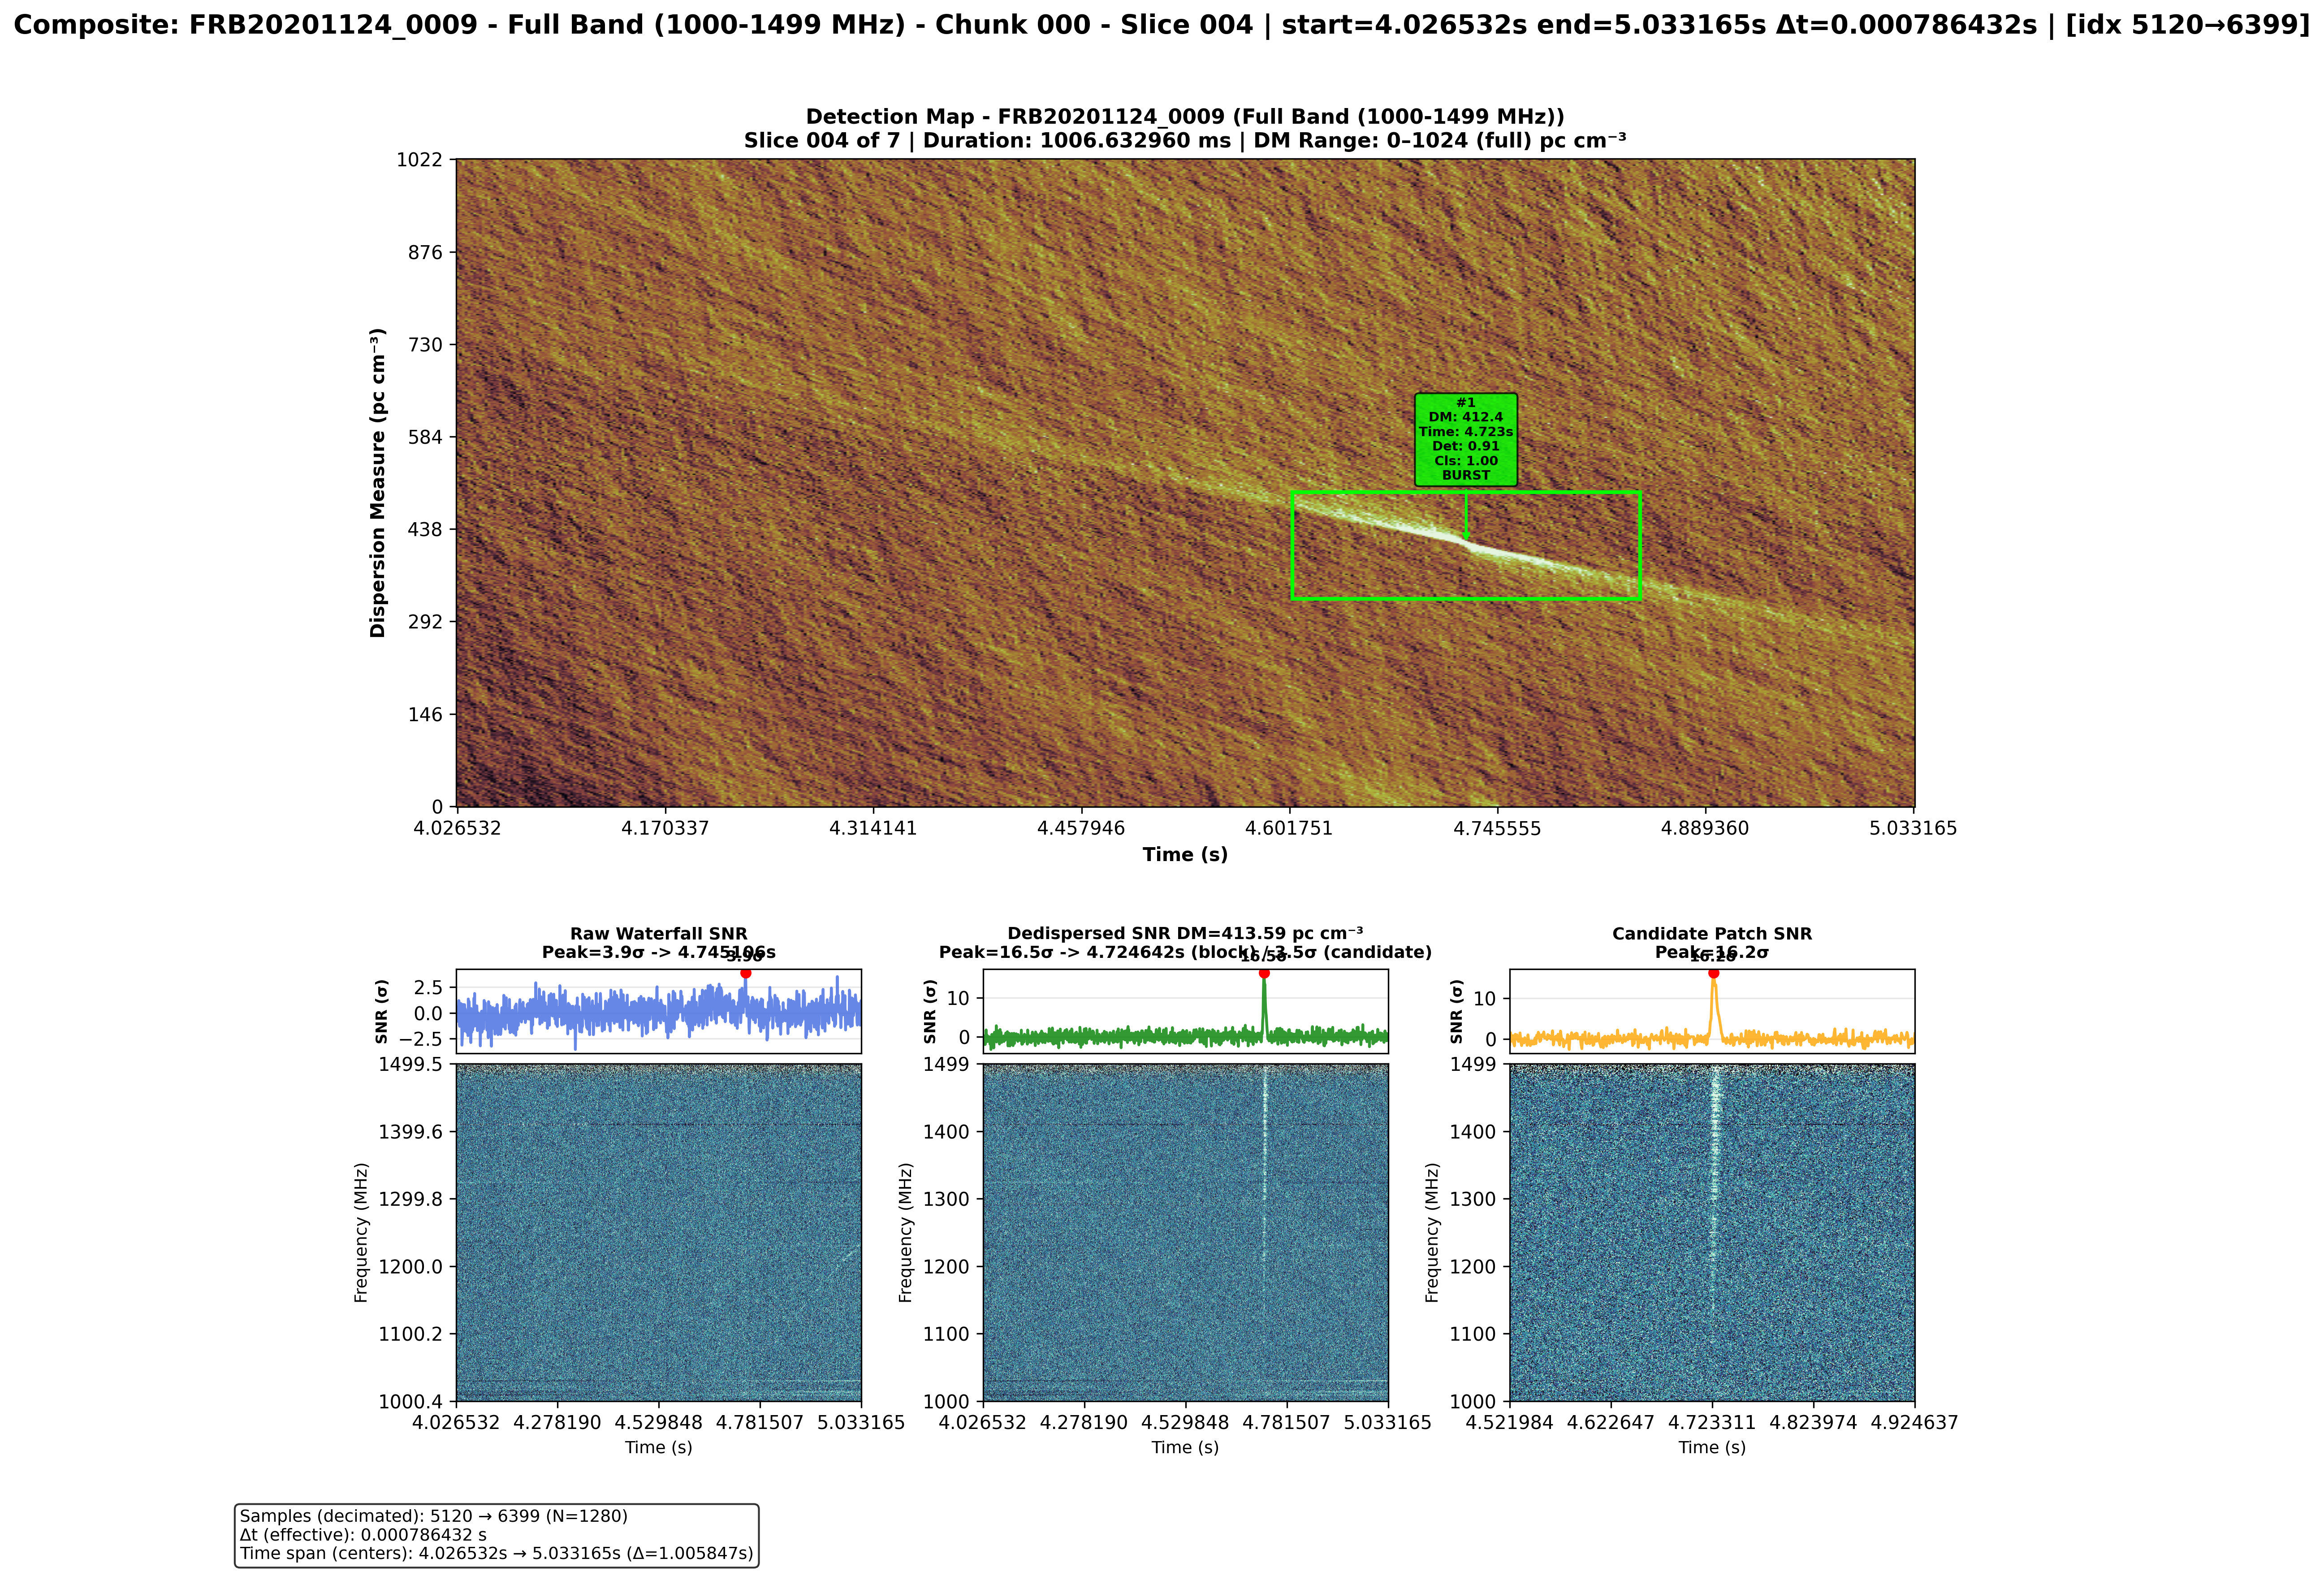
\includegraphics[width=\textwidth]{figures/Resultados/FAST-FREX/FRB20201124_0009_slice004.png}
    \caption[Validación funcional E2E: Segundo FRB (FAST-FREX) - Complementaria]{Figura~\ref{fig:anexo_frb20201124_0009_slice004}. Segunda detección de FRB (FAST, 1.25 GHz) con SNR=16.5$\sigma$. Mapa DM-tiempo muestra patrón dispersivo característico. Complementa la Figura~\ref{fig:frb20180301_0001_slice003} del Capítulo 5.}
    \label{fig:anexo_frb20201124_0009_slice004}
\end{figure}

\begin{figure}[H]
    \centering
    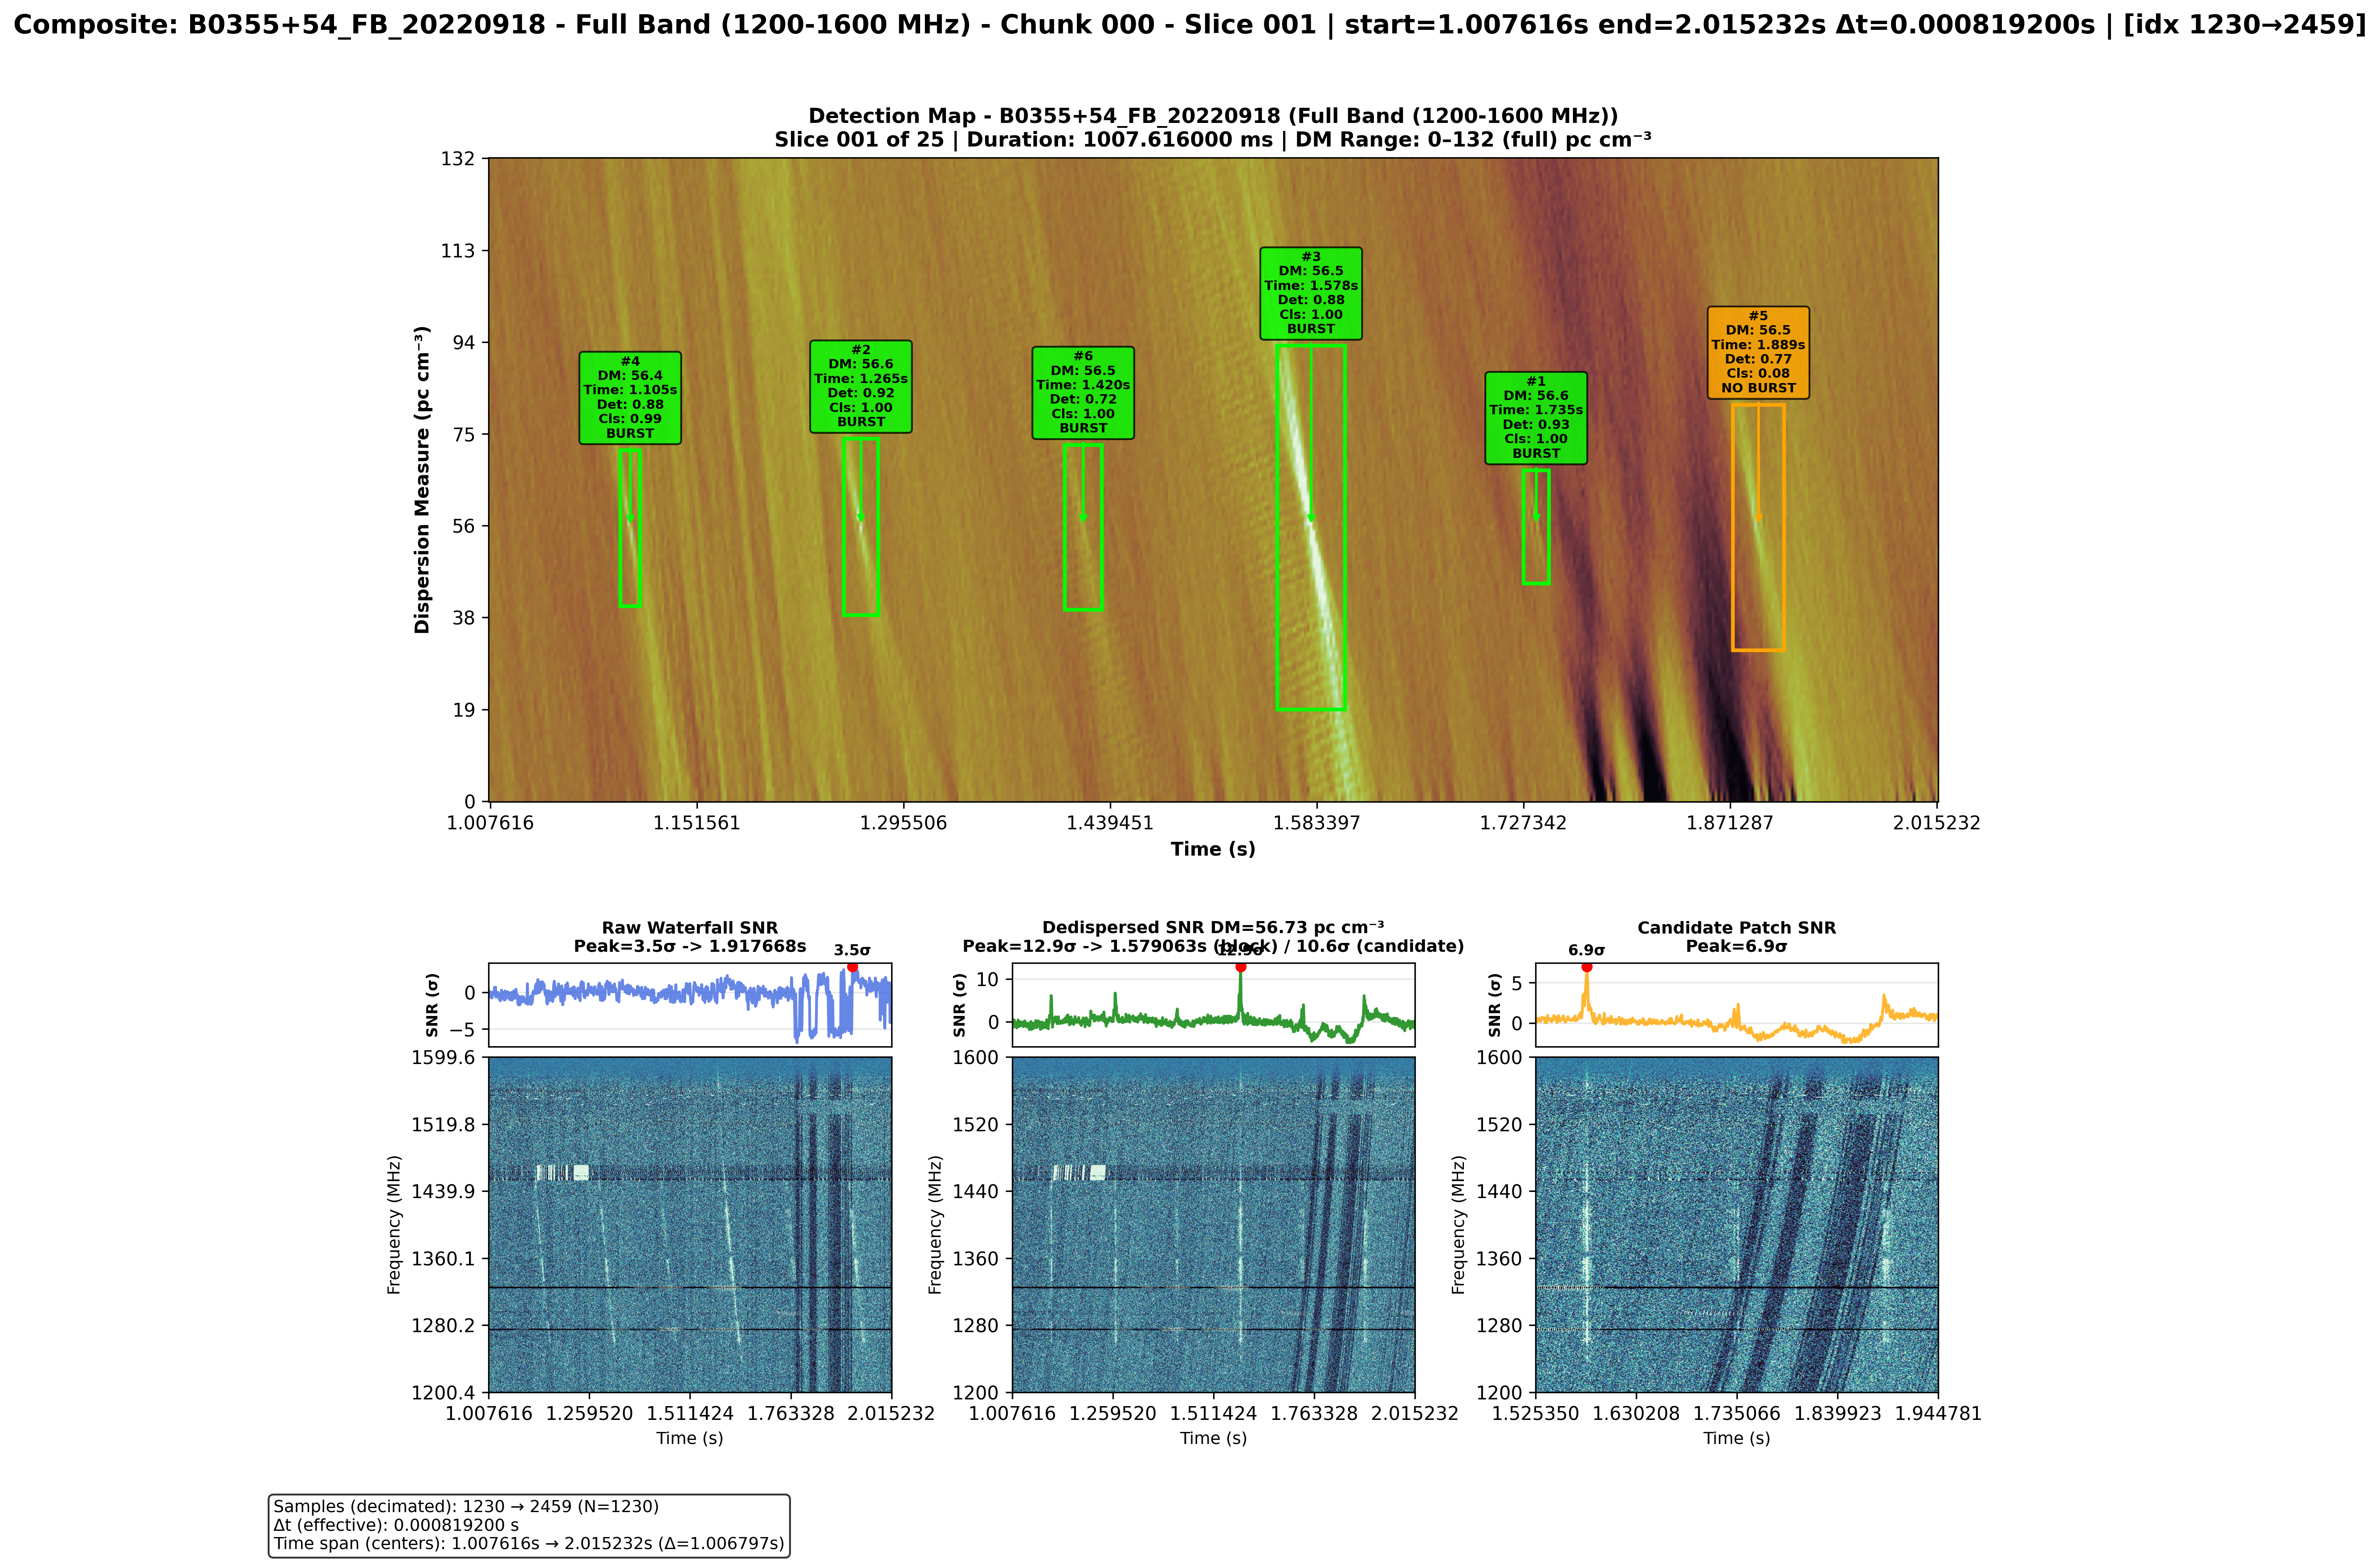
\includegraphics[width=\textwidth]{figures/Resultados/B0355+54/B0355+54_FB_20220918_slice001.png}
    \caption[Validación robustez temporal: Discriminación en Slice 001 - Complementaria]{Figura~\ref{fig:anexo_b0355_slice001}. Detección de 6 pulsos del púlsar B0355+54 (FAST, 1.25 GHz) en slice 001: 5 clasificados como BURST, 1 como NO BURST. Mapa DM-tiempo muestra variabilidad en clasificación. Complementa la Figura~\ref{fig:b0355_slice000} del Capítulo 5.}
    \label{fig:anexo_b0355_slice001}
\end{figure}

\begin{figure}[H]
    \centering
    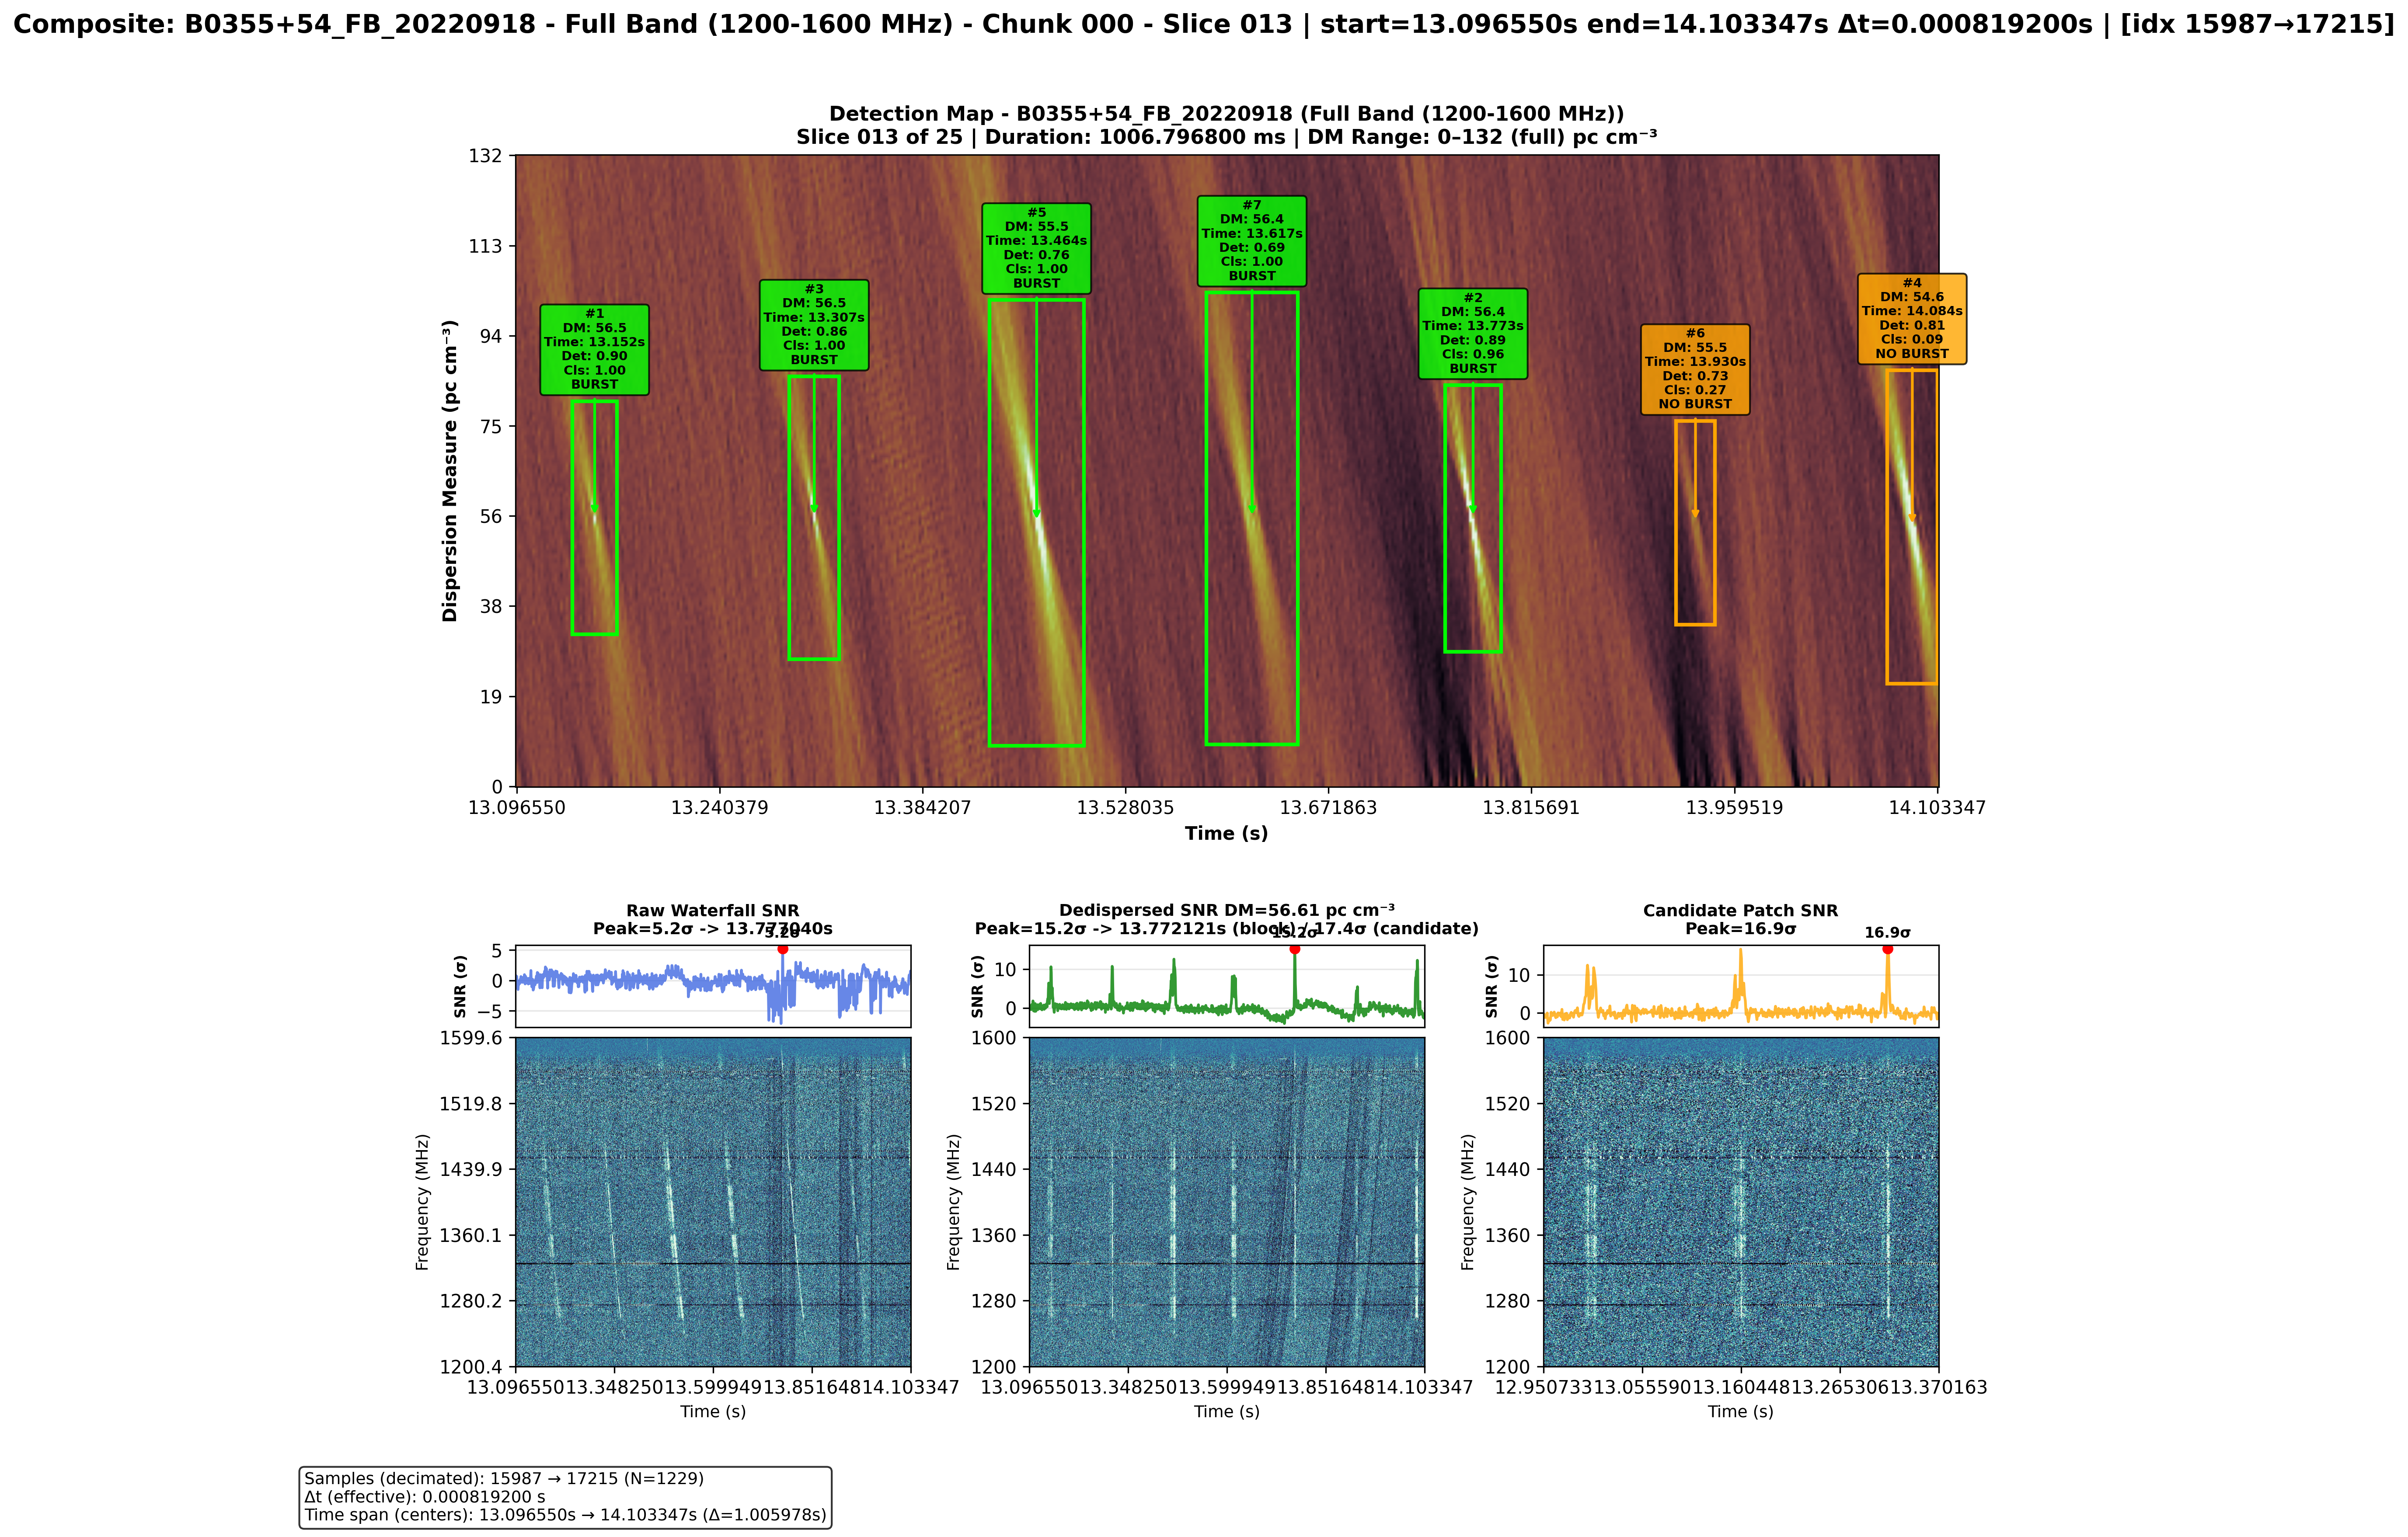
\includegraphics[width=\textwidth]{figures/Resultados/B0355+54/B0355+54_FB_20220918_slice013.png}
    \caption[Validación especificidad: Rechazo de señales ambiguas - Complementaria]{Figura~\ref{fig:anexo_b0355_slice013}. Eventos con alta detección (scores 0.73-0.81) pero baja clasificación (0.09-0.27) correctamente clasificados como NO BURST. Mapa DM-tiempo muestra rechazo de señales ambiguas. Complementa los resultados del Caso 2 del Capítulo 5.}
    \label{fig:anexo_b0355_slice013}
\end{figure}

\begin{figure}[H]
    \centering
    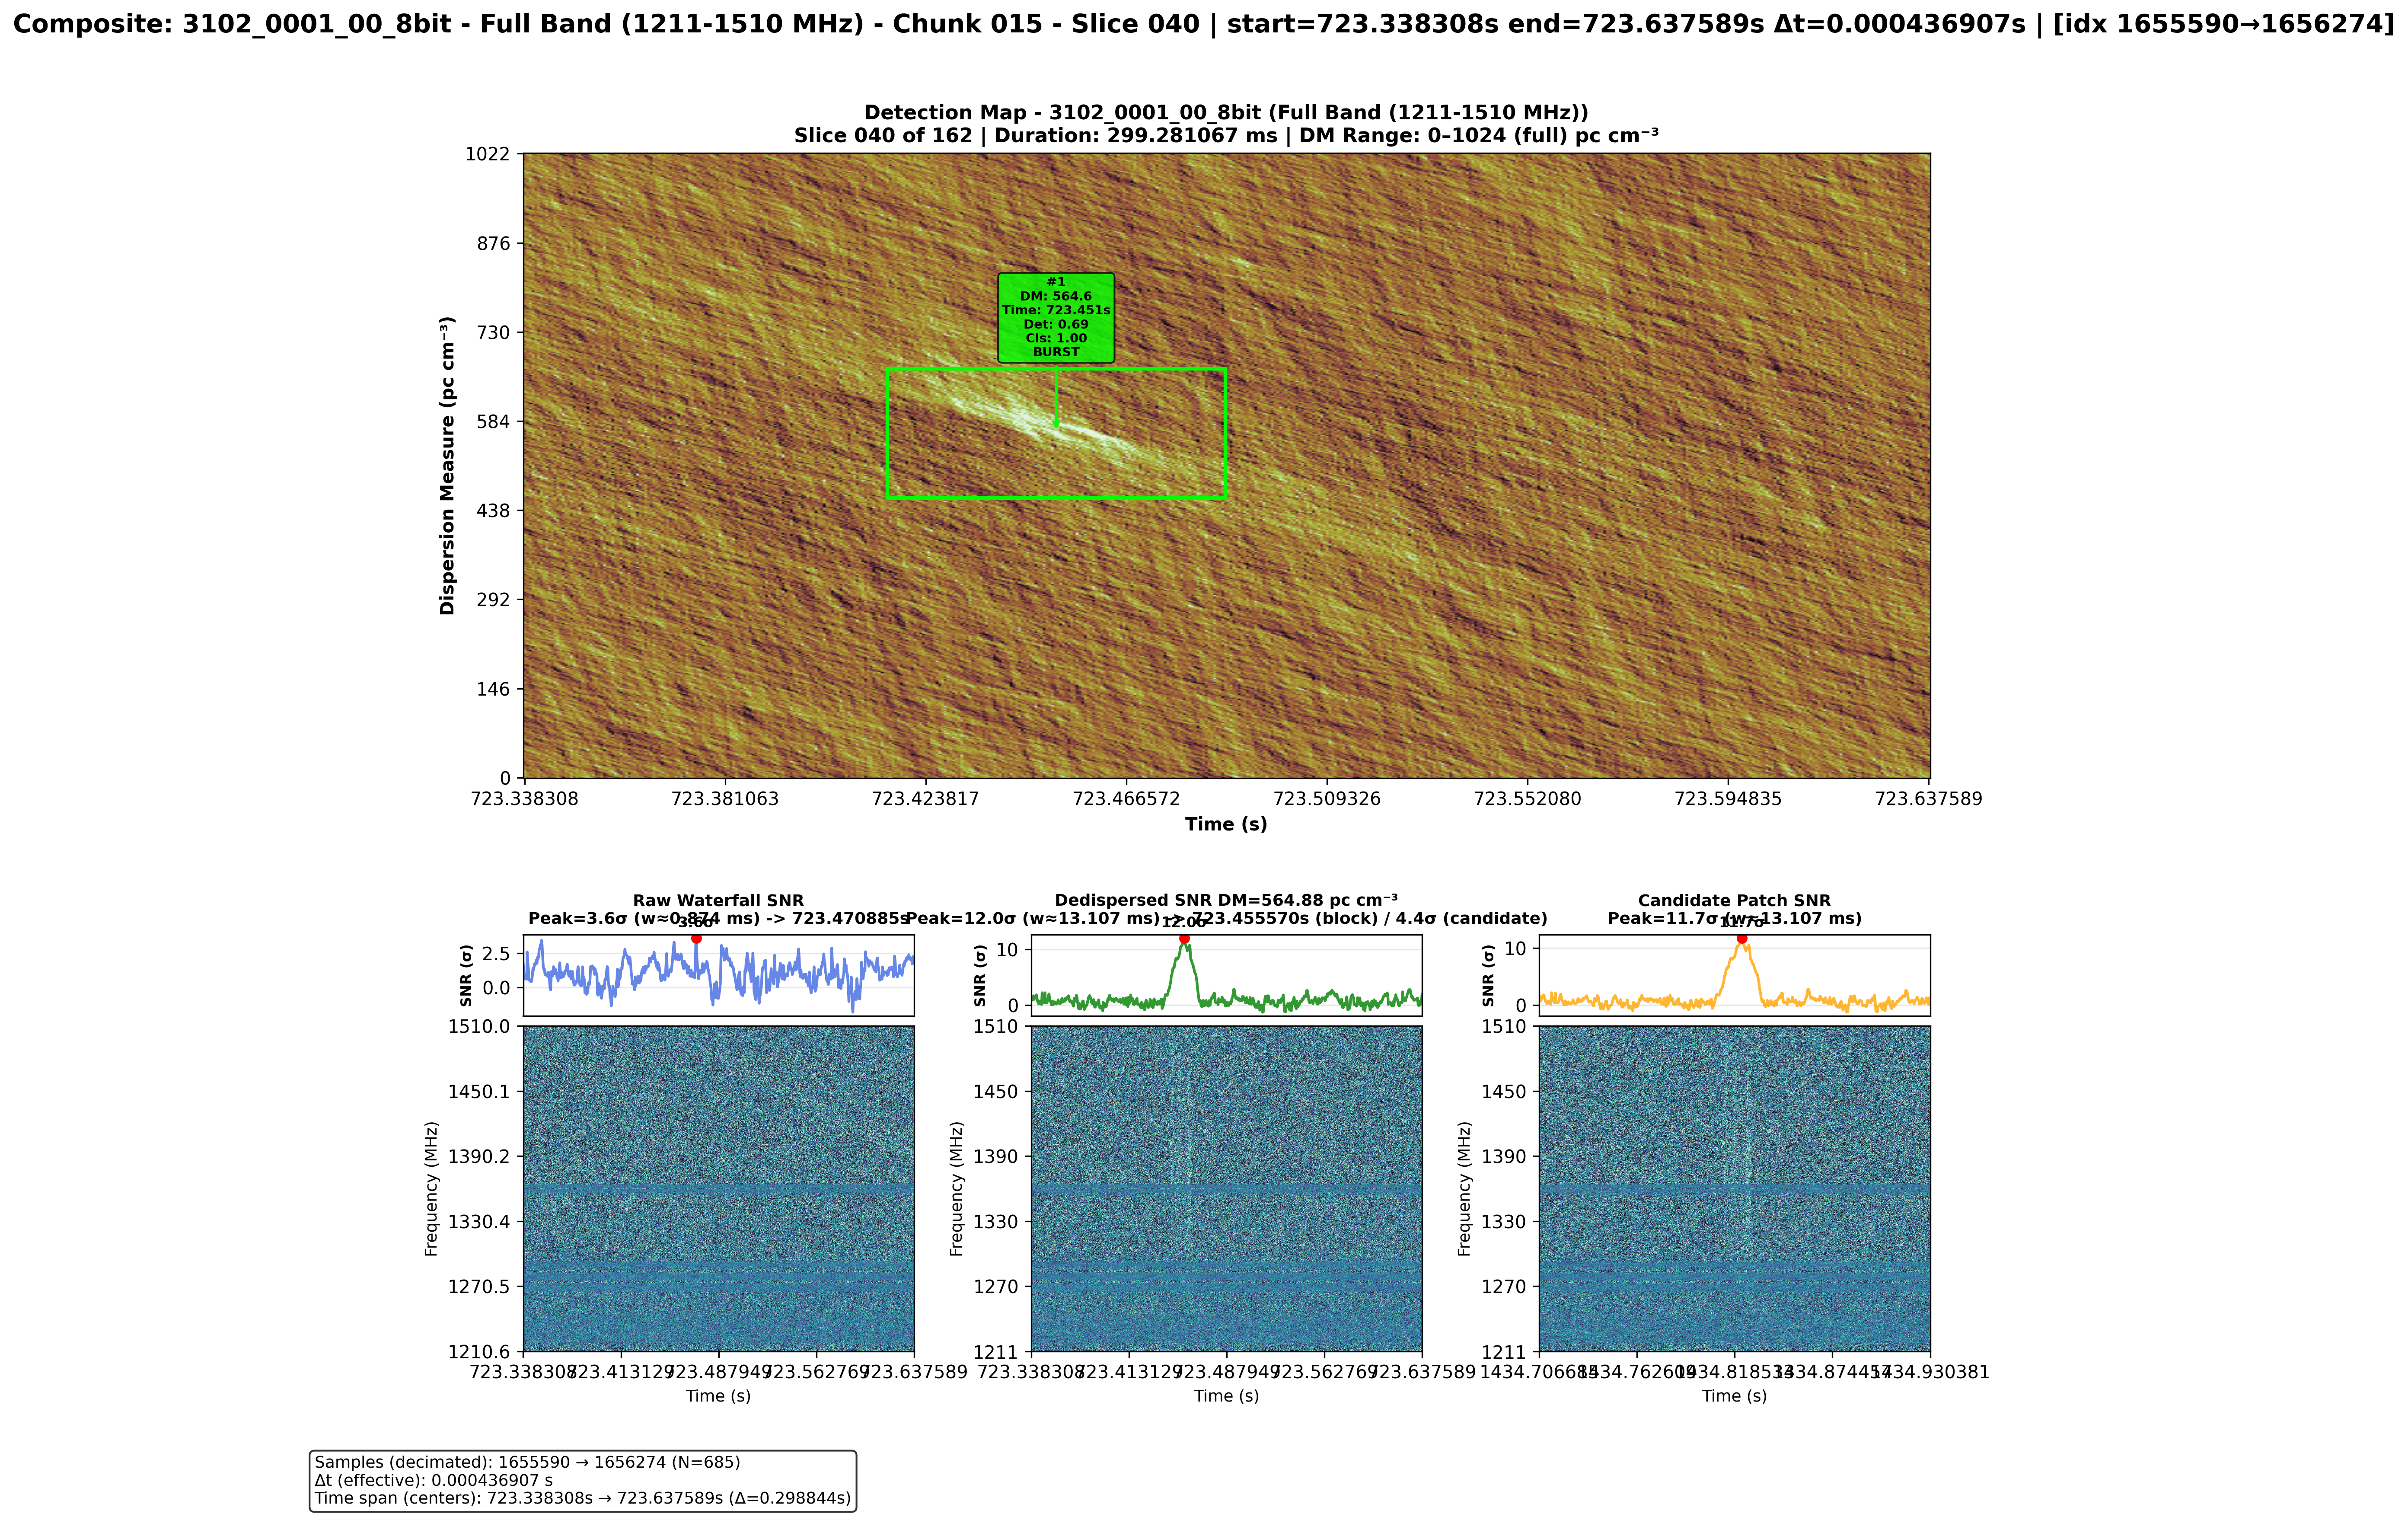
\includegraphics[width=\textwidth]{figures/Resultados/FRB121102/3102_0001_00_8bit_slice040.png}
    \caption[Descubrimiento científico: Segundo nuevo FRB 121102 - Complementaria]{Figura~\ref{fig:anexo_new_event_3102}. Segundo nuevo evento de FRB 121102 confirmado (Effelsberg, 1.4 GHz). Mapa DM-tiempo muestra detección en DM=564.88 pc cm$^{-3}$, t=723.5 s, SNR=12.0$\sigma$. Complementa la Figura~\ref{fig:new_event_3096} del Capítulo 5.}
    \label{fig:anexo_new_event_3102}
\end{figure}

\subsubsection{Figuras Complementarias - Línea 1 (Justificación)}

\begin{figure}[H]
    \centering
    \includegraphics[width=0.9\textwidth]{figures/Resultados/8 pulsos canonicos/2017-04-03-13_38_31_242_0005_t44.169_slice149.png}
    \caption[Justificación: Fallo Sistemático del Pipeline Clásico (Caso B, umbral conservador) - Complementaria]{Figura~\ref{fig:anexo_242_0005_slice149_highProb}. Fallo del pipeline clásico en alta frecuencia (ALMA, 86 GHz) con umbral conservador (DET\_PROB = 0.3). Mapa DM-tiempo muestra ausencia de detecciones para pulso confirmado en t=44.169 s. Complementa las Figuras~\ref{fig:142_0003_slice133_highProb} y~\ref{fig:142_0003_slice133_lowProb} del Capítulo 5.}
    \label{fig:anexo_242_0005_slice149_highProb}
\end{figure}

\begin{figure}[H]
    \centering
    \includegraphics[width=0.9\textwidth]{figures/DRAFTS-HF-Sin-Modificaciones/2017-04-03-13_38_31_242_0005_t44.169_slice149-lowProb.png}
    \caption[Justificación: Limitaciones Arquitecturales Irreductibles (Caso B, umbral sensible) - Complementaria]{Figura~\ref{fig:anexo_242_0005_slice149_lowProb}. Mismo pulso de la Figura~\ref{fig:anexo_242_0005_slice149_highProb} procesado con umbral sensible (DET\_PROB = 0.05). Mapa DM-tiempo muestra que el pulso permanece indetectable. Complementa las Figuras~\ref{fig:142_0003_slice133_highProb} y~\ref{fig:142_0003_slice133_lowProb} del Capítulo 5.}
    \label{fig:anexo_242_0005_slice149_lowProb}
\end{figure}

\subsubsection{Figuras Complementarias - Línea 2a (Solución Híbrida)}

\begin{figure}[H]
    \centering
    \includegraphics[width=0.95\textwidth]{figures/DRAFTS-HF-SNR/2017-04-03-12_56_05_230_0003_t36.548_slice121.png}
    \caption[Validación Línea 2a: Re-detección Exitosa de Pulso PRESTO - Complementaria]{Figura~\ref{fig:anexo_alma_presence_validation_1}. Re-detección de pulso PRESTO (ALMA, 86 GHz) mediante Línea 2a (matched filtering + ResNet18 en I). Mapa DM-tiempo muestra detección en t=36.548 s. Complementa la Figura~\ref{fig:alma_presence_validation_2} del Capítulo 5.}
    \label{fig:anexo_alma_presence_validation_1}
\end{figure}

\begin{figure}[H]
    \centering
    \includegraphics[width=0.95\textwidth]{figures/DRAFTS-HF-SNR/2017-04-03-08_16_13_0001_slice143.png}
    \caption[Descubrimiento Científico: Nuevo Pulso del Magnetar (Línea 2a) - Complementaria]{Figura~\ref{fig:anexo_alma_new_candidate_validation}. Nuevo candidato del magnetar PSR J1745-2900 (ALMA, 86 GHz) detectado por Línea 2a. Mapa DM-tiempo muestra detección en t=43.136 s, DM=46.9 pc cm$^{-3}$, score 1.00. Complementa los resultados de Línea 2a del Capítulo 5.}
    \label{fig:anexo_alma_new_candidate_validation}
\end{figure}

\begin{figure}[H]
    \centering
    \includegraphics[width=0.9\textwidth]{figures/Resultados/Pulsos ALMA SOLO DRAFTS/2017-04-03-12_47_05_0002_slice037.png}
    \caption[Capacidad de Resolución Temporal Fina: Continuación del Pulso Extendido (Slice 037) - Complementaria]{Figura~\ref{fig:anexo_slice037_multiple_detections}. Continuación del pulso extendido: 6 componentes adicionales en slice 037 (11.1-11.4 s). Mapa DM-tiempo muestra estructura temporal compleja. Complementa la Figura~\ref{fig:slice036_multiple_detections} del Capítulo 5, mostrando la secuencia completa de 13 componentes.}
    \label{fig:anexo_slice037_multiple_detections}
\end{figure}

\subsubsection{Figuras Complementarias - Línea 2b (Refinamiento Físico)}

\begin{figure}[H]
    \centering
    \includegraphics[width=0.95\textwidth]{figures/linea 2a/2017-04-03-08_16_13_0001_slice086.png}
    \caption[Deduplicación Inteligente mediante Clasificación Dual - Complementaria]{Figura~\ref{fig:anexo_linea2b_slice086_dedup}. Deduplicación de componentes temporales mediante clasificación dual I+L (Línea 2b, modo STRICT). Mapa DM-tiempo muestra dos candidatos cercanos; el sistema selecciona el de mayor coherencia polarimétrica. Complementa las Figuras~\ref{fig:linea2a_slice086} y~\ref{fig:linea2b_slice086_fp} del Capítulo 5.}
    \label{fig:anexo_linea2b_slice086_dedup}
\end{figure}

\begin{figure}[H]
    \centering
    \includegraphics[width=0.95\textwidth]{figures/linea 2a/2017-04-03-12_56_05_0001_slice102.png}
    \caption[Limitación de Especificidad: Múltiples Falsos Positivos Aceptados - Complementaria]{Figura~\ref{fig:anexo_linea2a_slice102}. Limitación de Línea 2a (solo I): slice 102 genera dos candidatos clasificados como BURST sin validación polarimétrica. Mapa DM-tiempo muestra falsos positivos aceptados. Complementa las Figuras~\ref{fig:linea2a_slice086} y~\ref{fig:linea2b_slice086_fp} del Capítulo 5.}
    \label{fig:anexo_linea2a_slice102}
\end{figure}

\begin{figure}[H]
    \centering
    \includegraphics[width=0.95\textwidth]{figures/linea 2a/2017-04-03-12_56_05_0001_slice102-FP.png}
    \caption[Éxito de Transfer Learning en Polarización: Filtrado Múltiple - Complementaria]{Figura~\ref{fig:anexo_linea2b_slice102_fp}. Éxito de Línea 2b (dual I+L): los mismos dos candidatos de la Figura~\ref{fig:anexo_linea2a_slice102} son rechazados tras clasificación dual. Mapa DM-tiempo muestra filtrado de falsos positivos. Complementa las Figuras~\ref{fig:linea2a_slice086} y~\ref{fig:linea2b_slice086_fp} del Capítulo 5.}
    \label{fig:anexo_linea2b_slice102_fp}
\end{figure}

\begin{figure}[H]
    \centering
    \includegraphics[width=0.95\textwidth]{figures/Resultados/Pulsos ALMA SOLO DRAFTS/2017-04-03-08_16_13_0002_slice101.png}
    \caption[Candidato Final Línea 2b: Coherencia Polarimétrica Validada (Candidato 2) - Complementaria]{Figura~\ref{fig:anexo_linea2b_candidate_2}. Candidato validado por clasificación dual I+L (Línea 2b, modo STRICT). Mapa DM-tiempo muestra pulso con clasificación BURST en ambas polarizaciones (archivo 08\_16\_13\_0002, slice 101). Complementa la Figura~\ref{fig:linea2b_candidate_1} del Capítulo 5.}
    \label{fig:anexo_linea2b_candidate_2}
\end{figure}

\begin{figure}[H]
    \centering
    \includegraphics[width=0.95\textwidth]{figures/Resultados/Pulsos ALMA SOLO DRAFTS/2017-04-03-12_47_05_0005_slice016.png}
    \caption[Candidato Final Línea 2b: Morfología Consistente (Candidato 3) - Complementaria]{Figura~\ref{fig:anexo_linea2b_candidate_3}. Candidato con morfología consistente en ambas polarizaciones (Línea 2b, modo STRICT). Mapa DM-tiempo muestra pulso clasificado como BURST en I+L (archivo 12\_47\_05\_0005, slice 016). Complementa la Figura~\ref{fig:linea2b_candidate_1} del Capítulo 5.}
    \label{fig:anexo_linea2b_candidate_3}
\end{figure}

\begin{figure}[H]
    \centering
    \includegraphics[width=0.95\textwidth]{figures/Resultados/Pulsos ALMA SOLO DRAFTS/2017-04-03-13_38_31_0003_slice081.png}
    \caption[Candidato Final Línea 2b: Coherencia Morfológica Polarimétrica (Candidato 4) - Complementaria]{Figura~\ref{fig:anexo_linea2b_candidate_4}. Candidato con coherencia morfológica polarimétrica validada (Línea 2b, modo STRICT). Mapa DM-tiempo muestra pulso clasificado como BURST en I+L (archivo 13\_38\_31\_0003, slice 081). Complementa la Figura~\ref{fig:linea2b_candidate_1} del Capítulo 5.}
    \label{fig:anexo_linea2b_candidate_4}
\end{figure}

\begin{figure}[H]
    \centering
    \fbox{\textit{[Figura de candidato 5 - Pendiente de generación]}}
    \caption[Línea 2b Candidato 5 - Complementaria]{Línea 2b Candidato 5: Pulso con clasificación BURST en I+L (modo STRICT). Pendiente de generación de figura y validación experta. Esta figura complementa la Figura~\ref{fig:linea2b_candidate_1} del Capítulo 5. \textit{Fuente: Elaboración propia}.}
    \label{fig:anexo_linea2b_candidate_5}
\end{figure}
